\section{Diagrama del proceso general del sistema}
En la Figura \ref{fig:proceso_general} se observa el diagrama del proceso general del sistema.
\\
Un diagrama de proceso sirve para representar de forma gráfica el flujo de un conjunto de actividades o tareas que se realizarán en el sistema. 
\\
En este diagrama se representa el conjunto de actividades que permite describir las funcionalidades principales del sistema.
\begin{figure}[H]
	\centering
	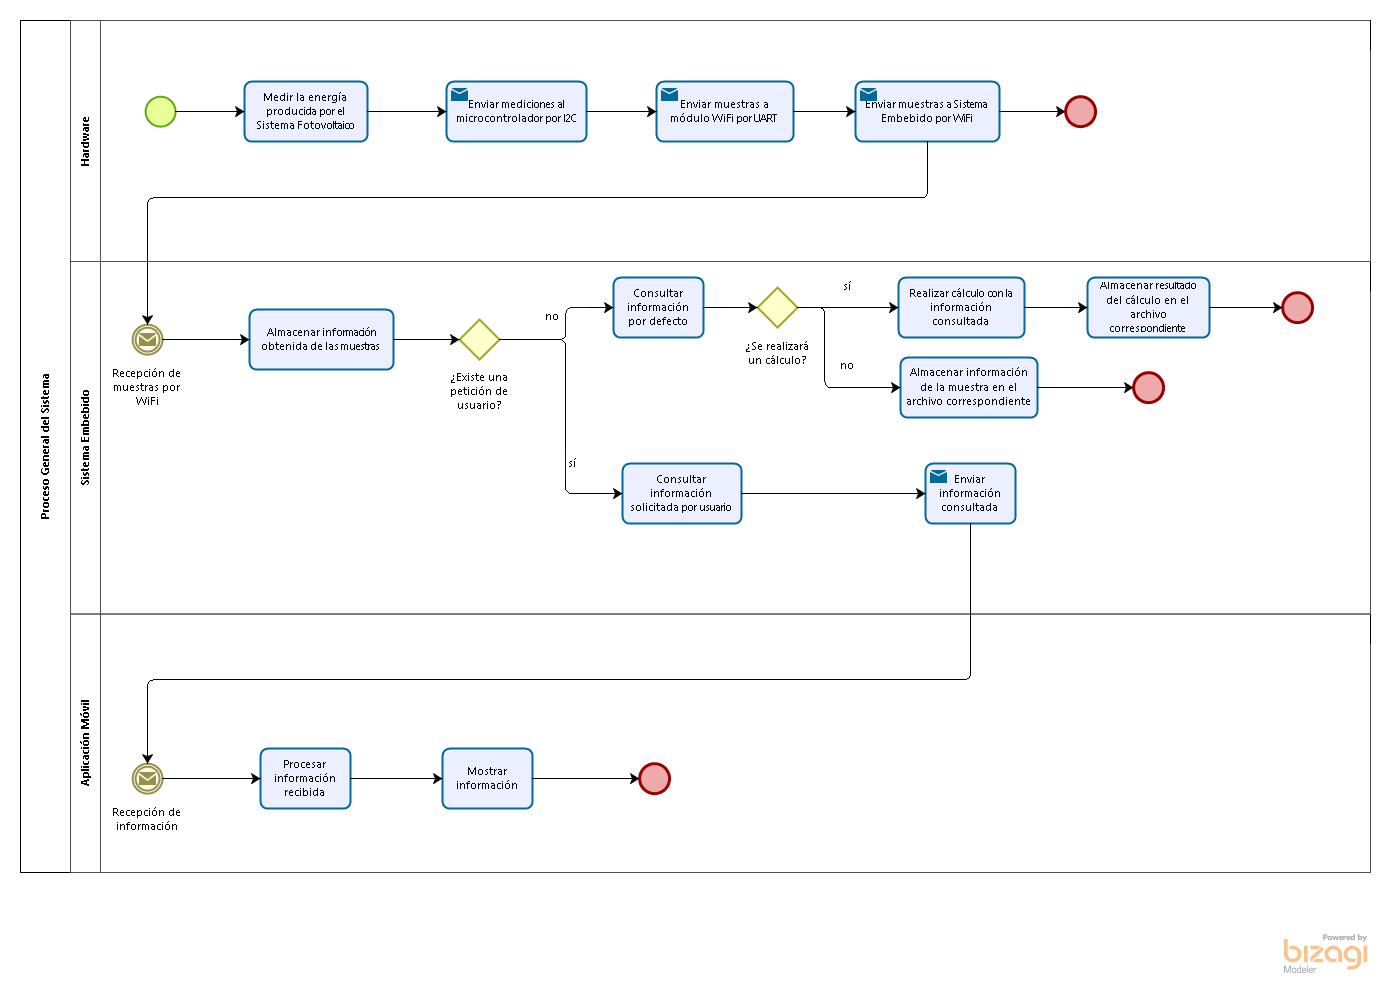
\includegraphics[scale=.48]{Capitulo4/images/procesoGeneral}
	\caption{Diagrama del proceso general del sistema}
	\label{fig:proceso_general}
\end{figure}
